\documentclass[submission,copyright,creativecommons]{eptcs}
\providecommand{\event}{QPL 2017} % Name of the event you are submitting to
\usepackage{breakurl}             % Not needed if you use pdflatex only.
\usepackage{underscore}           % Only needed if you use pdflatex.

\usepackage{amsfonts, amsthm, amssymb, amsmath, stmaryrd, etoolbox}
\usepackage{comment}
\usepackage{mathtools}
\usepackage{graphicx,caption,subcaption}
\usepackage{todonotes}
\usepackage{xcolor}
\usepackage{cite}

\usepackage[inline]{enumitem}
\setlist{itemsep=0em, topsep=0em, parsep=0em}
\setlist[enumerate]{label=(\alph*)}

\usepackage{tikz}
\usepackage[all,2cell]{xy}
\usetikzlibrary{matrix,arrows,shapes,decorations.markings,decorations.pathreplacing}
\definecolor{rewritecolor}{rgb}{0,.9,1}
\tikzset{rewritenode/.style={shape=circle,fill=rewritecolor,scale=0.25,font=\Huge}}
\tikzset{RWopen/.style={shape=circle,draw=black,fill=white,scale=0.5,font=\Huge}}
\tikzset{RWclosed/.style={shape=circle,fill=black,scale=0.5,font=\Huge}}
\tikzset{CDnode/.style={shape=circle,fill=white,scale=.5}}
\tikzset{zxgreen/.style={shape=circle,draw,thick,fill=green}}
\tikzset{zxred/.style={shape=circle,draw,thick,fill=red}}
\tikzset{zxyellow/.style={shape=rectangle,draw,thick,fill=yellow}}
\tikzset{zxdiamond/.style={shape=diamond,fill=black,inner sep=2.75}}
\tikzset{zxopen/.style={shape=circle,draw,thick,inner sep=2pt}}
\tikzset{->-/.style={decoration={%
			markings,
			mark=at position .5 with {\arrow{>}}},postaction={decorate}}
}
\tikzset{->-pos/.style={decoration={%
			markings,
			mark=at position #1 with {\arrow{>}}},postaction={decorate}}
}

\usepackage{hyperref}
\definecolor{hyperrefcolor}{rgb}{0,0,0.7}
\hypersetup{colorlinks,linkcolor={hyperrefcolor},citecolor={hyperrefcolor},urlcolor={hyperrefcolor}}

%NEW COMMANDS---------------------------------------------

\newcommand{\cl}[1]{\mathcal{#1}}
\newcommand{\scr}[1]{\mathscr{#1}}
\newcommand{\op}[1]{\operatorname{#1}}
\newcommand{\cat}[1]{\mathbf{#1}}
\newcommand{\dblcat}[1]{\mathbb{#1}}
\renewcommand{\t}[1]{\textup{#1}}

\newcommand{\from}{\colon}
\newcommand{\xto}[1]{\xrightarrow{#1}}
\newcommand{\sm}{\smallsetminus}
\newcommand{\tospan}{\xrightarrow{\mathit{sp}}}
\newcommand{\tocospan}{\xrightarrow{\mathit{csp}}}

%\newcommand{\diagram}[1]{\raisebox{-0.5\height}{\includegraphics{#1}}}

\newcommand{\bluebullet}{\textcolor{rewritecolor}{\bullet}}

%  macros for (co)span bicategories
\newcommand{\bispmap}[1]{\mathbf{Sp(#1)}}
\newcommand{\dblspmap}[1]{\mathbb{S}\mathbf{p(#1)}}
\newcommand{\bicspmap}[1]{\mathbf{Csp(#1)}}
\newcommand{\dblcspmap}[1]{\mathbb{C}\mathbf{sp(#1)}}
\newcommand{\bispsp}[1]{\mathbf{Sp(Sp(#1))}}
\newcommand{\dblspsp}[1]{\mathbb{S}\mathbf{p(Sp(#1))}}
\newcommand{\bicspcsp}[1]{\mathbf{Csp(Csp(#1))}}
\newcommand{\dblcspcsp}[1]{\mathbb{C}\mathbf{sp(Csp(#1))}}
\newcommand{\bimonspcsp}[1]{\mathbf{MonicSp(Csp(#1))}}
\newcommand{\dblmonspcsp}[1]{\mathbb{M}\mathbf{onicSp(Csp(#1))}}
\newcommand{\biepiccspsp}[1]{\mathbf{EpicCsp(Sp(#1))}}
\newcommand{\dblepiccspsp}[1]{\mathbb{E}\mathbf{picCsp(Sp(#1))}}
\newcommand{\bispcs}[1]{\mathbf{Sp}(\mathbf{Csp}(\mathbf{#1}))}
\newcommand{\hto}{\xslashedrightarrow{}}
\newcommand{\zx}{_{\text{zx}}}
\newcommand{\bicat}[1]{\underline{\mathbf{#1}}}
\newcommand{\SpCspZX}{\cat{Sp}(\cat{Csp}(\cat{Graph}\downarrow S_{\text{zx}}))}
\newcommand{\zxGraphs}{\cat{Graph} \downarrow S_{\text{zx}}}

% defining arrow with a vertical line through it
\makeatletter
\def\slashedarrowfill@#1#2#3#4#5{%
	$\m@th\thickmuskip0mu\medmuskip\thickmuskip\thinmuskip\thickmuskip
	\relax#5#1\mkern-7mu%
	\cleaders\hbox{$#5\mkern-2mu#2\mkern-2mu$}\hfill
	\mathclap{#3}\mathclap{#2}%
	\cleaders\hbox{$#5\mkern-2mu#2\mkern-2mu$}\hfill
	\mkern-7mu#4$%
}
\def\rightslashedarrowfill@{%
	\slashedarrowfill@\relbar\relbar\mapstochar\rightarrow}
\newcommand{\xslashedrightarrow}[2][]{%
	\ext@arrow 0055{\rightslashedarrowfill@}{#1}{#2}}
\makeatother

%DECLARE MATH OPERATORS----------------------------------

\DeclareMathOperator{\Hom}{Hom}
\DeclareMathOperator{\id}{id}
\DeclareMathOperator{\ob}{Ob}
\DeclareMathOperator{\arr}{arr}
\DeclareMathOperator{\im}{im}
\DeclareMathOperator{\Aut}{Aut}
\DeclareMathOperator{\Bij}{Bij}
\DeclareMathOperator{\Sub}{Sub}
\DeclareMathOperator{\decat}{decat}

%TITLE PAGE----------------------------------


\title{Categorifying the zx-calculus}
\author{Daniel Cicala
	\institute{Department of Mathematics\\
	University of California, Riverside\\
	USA}
	\email{cicala@math.ucr.edu}
}
\def\titlerunning{Categorifying the zx-calculus}
\def\authorrunning{Daniel Cicala}

\begin{document}
\maketitle

%\begin{abstract}
%	This paper presents a symmetric monoidal and compact closed bicategory that categorifies the zx-calculus developed by Coecke and Duncan.  The $1$-cells in this bicategory are certain graph morphisms that correspond to the string diagrams of the zx-calculus, while the $2$-cells are rewrite rules. 
%\end{abstract}

Compositionality is becoming increasingly recognized as a viable method to model complex systems such as those found in physics, computer science, and biology.  The idea is to study smaller, simpler systems and ways of connecting them together.  The word \emph{compositionality} suggests that category theory can play a key role, and indeed it does.  Systems are morphisms and connections are morphism composition.   

This paper \cite{CicalaCatZxCalc} looks at one example of compositionality in action: the zx-calculus.  The backstory dates to Penrose's tensor networks and, more recently, to the relationship between graphical languages and monoidal categories explored by Joyal, Street, and Selinger.  Abramsky and Coecke capitalized on this relationship when inventing a categorical framework for quantum physics \cite{AbramCoekeCatSemQuanProt}.  Through this perspective, Coecke and Duncan presented early results on a diagrammatic language in which to reason about \emph{complementary quantum observables}. After a fruitful period of development, the first complete presentation of the zx-calculus was published \cite{CoeckeDuncanInterQuanObs}. 

The zx-calculus begins with the wire, green spider, red spider, Hadamard, and diamond diagrams 
\begin{equation}
\raisebox{-1em}{%
	\raisebox{0.5em}{%
	\begin{tikzpicture} % generator wire
		\begin{scope}
		\node (1) at (0, 0) {};
		\node (2) at (1,0) {};
		\end{scope}
		\begin{scope}
		\draw [thick] (2.center) to (1.center);
		\node at (0,-.2) {};
		\end{scope}
	\end{tikzpicture}
}
%
%
\quad \quad \quad
%
%
	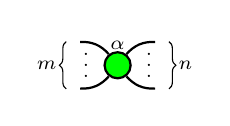
\begin{tikzpicture} % generator green spider
		\node [zxgreen,label={[shift={(0,-0.1)}]\scriptsize $\alpha$}] (v1) at (0,0) {};
		\node (v2) at (-0.6,0.3) {};
		\node (v3) at (-0.6,-0.3) {};
		\node (v4) at (0.6,0.3) {};
		\node (v5) at (0.6,-0.3) {};
		\node at (-0.4,0.1) {\scriptsize $\vdots$};
		\node at (0.4,0.1) {\scriptsize $\vdots$};
		\draw  (v1) edge [thick,bend right=25] (v2);
		\draw  (v1) edge [thick,bend left=25] (v3);
		\draw  (v1) edge [thick,bend left=25] (v4);
		\draw  (v1) edge [thick,bend right=25] (v5);
		\draw[decoration={brace,mirror,raise=5pt},decorate]
		(v2.east) -- node[left=5pt] {\scriptsize $m$} (v3.east); 
		\draw[decoration={brace,raise=5pt},decorate]
		(v4.west) -- node[right=5pt] {\scriptsize $n$} (v5.west); 
	\end{tikzpicture}
%
%
\quad \quad \quad
%
%
	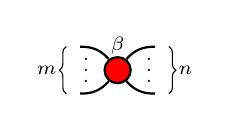
\begin{tikzpicture} % generator red spider
		\node [zxred,label={[shift={(0,-0.1)}]\scriptsize $\beta$}] (v1) at (0,0) {};
		\node (v2) at (-0.6,0.3) {};
		\node (v3) at (-0.6,-0.3) {};
		\node (v4) at (0.6,0.3) {};
		\node (v5) at (0.6,-0.3) {};
		\node at (-0.4,0.1) {\scriptsize $\vdots$};
		\node at (0.4,0.1) {\scriptsize $\vdots$};
		%
		\draw  (v1) edge [thick,bend right=25] (v2);
		\draw  (v1) edge [thick,bend left=25] (v3);
		\draw  (v1) edge [thick,bend left=25] (v4);
		\draw  (v1) edge [thick,bend right=25] (v5);
		\draw[decoration={brace,mirror,raise=5pt},decorate]
		(v2.east) -- node[left=5pt] {\scriptsize $m$} (v3.east); 
		\draw[decoration={brace,raise=5pt},decorate]
		(v4.west) -- node[right=5pt] {\scriptsize $n$} (v5.west); 
	\end{tikzpicture}
%
%
\quad \quad \quad
%
%
	\raisebox{0.75em}{%
	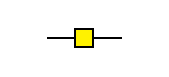
\begin{tikzpicture} % generator hadarmard
		\node [zxyellow] (v1) at (0,0) {};
		\node (v2) at (-0.6,0) {};
		\node (v3) at (0.6,0) {};
		\draw  (v1) edge [thick] (v2);
		\draw  (v1) edge [thick] (v3);
	\end{tikzpicture}
}
%
%
\quad \quad \quad
%
%
	\raisebox{0.5em}{%
	
\begin{tikzpicture} % generator diamond
		\node [zxdiamond] () at (0,0) {};
	\end{tikzpicture}
}
}
\end{equation}
Observe that there are dangling wires on the left and right. Think of those on the left as inputs and those on the right as outputs. A pair of diagrams are composable when the inputs of one match the outputs of another.  Formalizing this perspective, we let these diagrams generate the morphisms of a dagger compact category $\mathbf{zx}$ whose objects are the non-negative integers.  The meaning of these objects is to give the number of inputs and outputs for a morphism $n \to m$.  These morphisms are then subjected to a number of relations which are listed in full in the preprint \cite{CicalaCatZxCalc}.  For illustrative purposes, we will present one of the relations:
\begin{equation}
\label{diag:spider relation}
\raisebox{-3.5em}{%
	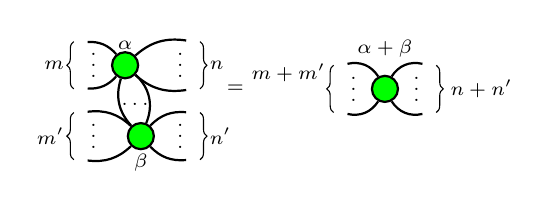
\begin{tikzpicture}
	%
	%
	%
	\begin{scope}[shift={(-0.2,0)}] 
	\node [zxgreen,label={[shift={(0,-0.1)}]\scriptsize $\alpha$}] (000) at (-0.3,1.2) {};
	\node [zxgreen,label={[shift={(0,-0.75)}] \scriptsize $\beta$}] (001) at (-0.1,0.3) {};
	\node (v1) at (-0.9,1.5) {};
	\node (v2) at (-0.9,0.9) {};
	\node (v3) at (-0.9,0.6) {};
	\node (v4) at (-0.9,0) {};
	\draw  (000) edge[thick,bend right=25] (v1);
	\draw  (000) edge[thick,bend left=25] (v2);
	\draw  (001) edge[thick,bend right=25] (v3);
	\draw  (001) edge[thick,bend left=25] (v4);
	%
	\node (v5) at (0.6,1.5) {};
	\node (v6) at (0.6,0.9) {};
	\node (v7) at (0.6,0.6) {};
	\node (v8) at (0.6,0) {};
	\draw  (000) edge[thick,bend left=25] (v5);
	\draw  (000) edge[thick,bend right=25] (v6);
	\draw  (001) edge[thick,bend left=25] (v7);
	\draw  (001) edge[thick,bend right=25] (v8); 
	%
	\node (d3) at (0.4,1.3) {\scriptsize $\vdots$};
	\node (d4) at (0.4,0.4) {\scriptsize $\vdots$};
	\node (d5) at (-0.7,1.3) {\scriptsize $\vdots$};
	\node (d5) at (-0.7,0.4) {\scriptsize $\vdots$};
	\node at (-0.15,0.7) {\scriptsize $\dots$};
	\draw  (000) edge[thick,bend right=30] (001);
	\draw  (000) edge[thick,bend left=35] (001);
	\draw[decoration={brace,mirror,raise=5pt},decorate]
	(v1.east) -- node[left=5pt] {\scriptsize $m$} (v2.east); 
	\draw[decoration={brace,mirror,raise=5pt},decorate]
	(v3.east) -- node[left=5pt] {\scriptsize $m'$} (v4.east); 
	\draw[decoration={brace,raise=5pt},decorate]
	(v5.west) -- node[right=5pt] {\scriptsize $n$} (v6.west); 
	\draw[decoration={brace,raise=5pt},decorate]
	(v7.west) -- node[right=5pt] {\scriptsize $n'$} (v8.west); 
	\end{scope}
	%
	%
	%
	\node (equal) at (0.9,0.9) {\scriptsize $=$};
	%
	%
	%
	\begin{scope}[shift={(0.4,0)}]
	\node [zxgreen,label={[shift={(0,0.1)}]\scriptsize $\alpha+\beta$}] (000) at (2.4,0.9) {};
	\node (v9) at (1.8,1.2) {};
	\node (v10) at (1.8,0.6) {};
	\node (v11) at (3,1.2) {};
	\node (v12) at (3,0.6) {};
	\node (d1) at (2,1) {\scriptsize $\vdots$};
	\node (d2) at (2.8,1) {\scriptsize $\vdots$};
	%
	\draw  (000) edge[thick,bend right=35] (v9);
	\draw  (000) edge[thick,bend left=35] (v10);
	\draw  (000) edge[thick,bend left=35] (v11);
	\draw  (000) edge[thick,bend right=35] (v12);
	\draw[decoration={brace,mirror,raise=5pt},decorate]
	(v9.east) -- node[shift={(-.75,0.2)}] {\scriptsize $m+m'$} (v10.east); 
	\draw[decoration={brace,raise=5pt},decorate]
	(v11.west) -- node[shift={(.75,0)}] {\scriptsize $n+n'$} (v12.west); 
	\end{scope}
	\end{tikzpicture}
}
\end{equation}

Our main result is the construction of a symmetric monoidal and compact closed bicategory $\bicat{zx}$ that categorifies the dagger compact category $\cat{zx}$. The process of building $\bicat{zx}$ begins with (directed) graphs and adding additional structure that mimics the $\cat{zx}$-morphisms.

The first difference between graphs and $\cat{zx}$-morphisms we recognize is that the former have single-sorted nodes while the latter have multi-sorted nodes. We address this by considering the graph $S\zx$
\[
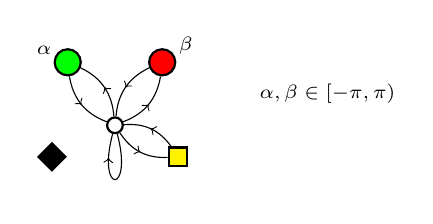
\begin{tikzpicture}
\node [zxopen] (v1) at (0,0) {};
\node [zxgreen,label={[shift={(-.3,-.2)}]\scriptsize $\alpha$}] (v2) at (-0.6,0.8) {};
\node [zxyellow] (v3) at (0.8,-0.4) {};
\node [zxdiamond] (v5) at (-0.8,-0.4) {};
\node [zxred,label={[shift={(.3,-.2)}]\scriptsize $\beta$}] (v4) at (0.6,0.8) {};
\node at (2.7,0.4) {\scriptsize $\alpha, \beta \in [-\pi,\pi)$};
%
\draw [->-] (v1) to [bend right] (v2);
\draw [->-] (v2) to [bend right] (v1);
\draw [->-] (v1) to [bend right] (v3);
\draw [->-] (v3) to [bend right] (v1);
\draw [->-] (v1) to [bend right] (v4);
\draw [->-] (v4) to [bend right] (v1);
\draw [->-pos=0.75]  (v1) to [loop below, looseness=35] (v1);
\end{tikzpicture}
\]
Note that there is a red and green node for each number in $[-\pi, \pi)$, all of which have a single edge to and from the white node. The idea is that $S\zx$ will classify nodes of a graph $G$ is by considering morphisms $G \to S\zx$.  Then each node of $G$ is colored according to whichever fiber it inhabits.  It should be clear how the fibers of each $S\zx$-node sorts the $G$-nodes in a way that matches the sorting of the $\cat{zx}$-morphisms, except perhaps for the white node.  Because graph edges must be attached to nodes at both ends, the white-sorted nodes serve as the analogue to the dangling input and output wires of $\cat{zx}$-morphisms. To illustrate, here is a graph over $S\zx$ corresponding to the green spider $\cat{zx}$-morphism:
\[
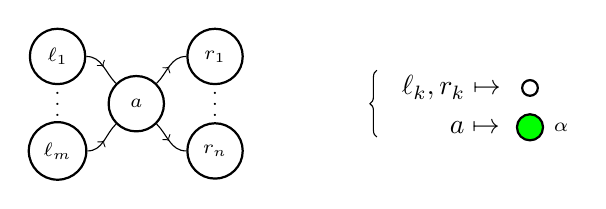
\begin{tikzpicture}
\begin{scope}[shift={(-1,3.2)}]
\begin{scope}[shift={(0,0)}]
\node [circle,draw,thick,minimum size=20pt] (a) at (0,0) {\scriptsize $a$}; 
\node [circle,draw,thick,minimum size=20pt] (1l) at (-1,0.6) {\scriptsize $\ell_1$};
\node [circle,draw,thick,minimum size=20pt] (m) at (-1,-0.6) {\scriptsize $\ell_m$};
\node at (-1,0.1) {\scriptsize $\vdots$};
\node [circle,draw,thick,minimum size=20pt] (1r) at (1,0.6) {\scriptsize $r_1$};
\node [circle,draw,thick,minimum size=20pt] (n) at (1,-0.6) {\scriptsize $r_n$};
\node at (1,0.1) {\scriptsize $\vdots$};
%
\draw [->-] (1l) to [out=0,in=135] (a);
\draw [->-] (m) to [out=0,in=-135] (a);
\draw [->-] (a) to [out=45,in=180] (1r);
\draw [->-] (a) to[out=-45,in=180] (n);
\end{scope}
\begin{scope}[shift={(4,0.2)}]
\node at (0,0) {$\ell_k, r_k \mapsto$};
\node at (0.3,-0.5) {$a \mapsto$};
\node [zxopen] at (1,0) {};
\node [zxgreen,label={[label distance=0pt]0:\scriptsize $\alpha$}] (3) at (1,-0.5) {};
\node (1) at (-0.75,0.1) {};
\node (2) at (-0.75,-0.5) {};
\draw [decoration={brace,mirror,raise=2pt},decorate] (1.north west) -- (2.south west); 	
\end{scope}
\end{scope}
\end{tikzpicture}
\]
We point out that graphs over $S\zx$ are merely objects in the over category $\cat{Graph} \downarrow S\zx$.  

Having introduced structure that correctly sorts the node, we now look to compose graphs over $S\zx$ as we did $\cat{zx}$-morphisms.  For this, we must somehow declare certain nodes to be inputs and outputs.  In particular, the inputs and outputs must only be chosen from the white nodes, as they correspond to the dangling wires.  To provide this structure, define a functor $N\zx \from \text{skel}(\cat{Set}) \to \cat{Graph} \downarrow S\zx$ on a skeleton of $\cat{Set}$ by letting $N\zx (X)$ be the edgeless graph with node set $X$ that is constant over the white node.   Then a graph over $S\zx$ with inputs and outputs, or an \emph{open graph over $S\zx$} can be defined as a cospan of the form
\[
	N\zx (X) \to G \gets N\zx (Y)
\]
in $\cat{Graph} \downarrow S\zx$.  The left and right legs of the cospan choses inputs and outputs, respectively, of $G$. Composition is achieved via pushout
\[
	\left( N(X)\zx \to G \gets N(Y)\zx \right) ; 
	\left( N(Y)\zx \to G' \gets N(Z)\zx \right) =
	\left( N(X)\zx \to G +_{N(Y)} G'\zx \gets N\zx(Z) \right).
\]

Taking a quick step back, it was shown in \cite{CicalaSpansOfCospan} that given any topos $\cat{T}$, there is a bicategory $\bispcs{T}$ with $\cat{T}$-objects as $0$-cells, cospans in $\cat{T}$ as $1$-cells, and isomorphism classes of monic spans of cospans as $2$-cells. A monic span of cospans  and their morphisms are the respective commuting diagrams in $\cat{T}$
\[
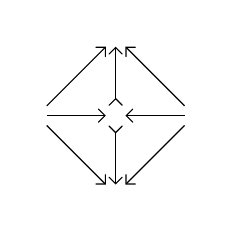
\begin{tikzpicture}
\node (A) at (0,0) {};
\node (B) at (1,1) {};
\node (B') at (1,0) {};
\node (B'') at (1,-1) {};
\node (C) at (2,0) {};
%
\path[->,font=\scriptsize,>=angle 90]
(A) edge node[above]{$$} (B)
(A) edge node[above]{$$} (B')
(A) edge node[above]{$$} (B'')
(C) edge node[above]{$$} (B)
(C) edge node[above]{$$} (B')
(C) edge node[left]{$$} (B'')
(B') edge[>->] node[right]{$$} (B)
(B') edge[>->] node[left]{$$} (B'');
\end{tikzpicture}
%
\quad \quad \quad \quad 
%
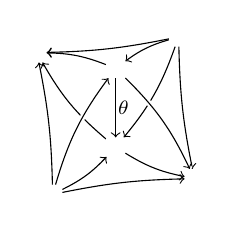
\begin{tikzpicture}
\node (1) at (-0.2,-1.6) {};
\node (2) at (-0.4,0.2) {};
\node (3) at (1.4,0.4) {};
\node (4) at (1.6,-1.4) {};
\node (5) at (0.6,0) {};
\node (6) at (0.6,-1) {};
%
\draw [->] (1) to[bend left=-5] (2);
\draw [->] (1) to[bend left=5] (4);
\draw [->] (1) to[bend left=-10] (6);
\draw [->] (3) to[bend left=5] (2);
\draw [->] (3) to[bend left=-5] (4);
\draw [->] (3) to[bend left=-10] (5);
\draw [->] (3) to[bend left=10] (6);
\draw [->] (5) to[bend left=-10] (2);
\draw [->] (6) to[bend left=10] (2);
\draw [->] (6) to[bend left=-10] (4);
\draw [->] (5) to[] node [shift={(0.1,0)}] {\scriptsize $\theta$} (6);

\draw [-,line width=0.2em,white] (1) to[bend left=10] (5);
\draw [->] (1) to[bend left=10] (5);
\draw [-,line width=0.2em,white] (5) to[bend left=10] (4);
\draw [->] (5) to[bend left=10] (4);
\end{tikzpicture}
\]
where `$\rightarrowtail$' is monic. In a joint paper by the author and Courser \cite{CicalaCourserBicatsSpanCospans}, it was shown that this bicategory is symmetric monoidal and compact closed.  However, to ensure in our final construction that the wire $\cat{zx}$-morphism behaves as an identity on $1$, we modify the above construction to take as $2$-cells the \emph{morphism classes} of spans of cospans. That is, we identify spans of cospans according to the equivalence classes generated by the relation $(\phi, \psi)$ if there is a morphism of spans of cospans $\phi \to \psi$.  This still results in a symmetric monoidal and compact closed bicategory, as shown in \cite{CicalaCatZxCalc}. 

Taking $\cat{T}$ to be the topos $\cat{Graph} \downarrow S\zx$, we consider the 1-full and 2-full sub-bicategory $\cat{zxRewrite}$ of $\bispcs{T}$ on the objects in the image of $N\zx$.   The $1$-cells in $\cat{zxRewrite}$ are exactly the open graphs over $S\zx$ and the $2$-cells are double pushout rewrite rules.  The generating $\cat{zx}$-morphisms can be realized in this scenario as the $1$-cells
\[
% 
% wire diagram
%
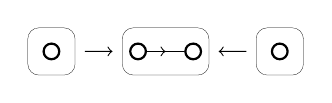
\begin{tikzpicture}
\begin{scope}[shift={(-0.2,-0.1)}]
\node [zxopen] (v2) at (1,-0.5) {};
\node (v11) at (1.3,-0.5) {};
\draw [ultra thin, rounded corners] (0.7,-0.2) rectangle (1.3,-0.8);
\end{scope}
%
\begin{scope}[shift={(4.8,0.1)}]
\node [zxopen] (v1) at (-2.2,-0.7) {};
\node [zxopen] (v2) at (-2.9,-0.7) {};
\draw [->-] (v2) to (v1);
\draw [ultra thin, rounded corners] (-3.1,-0.4) rectangle (-2,-1);
\node (v12) at (-3.1,-0.7) {};
\node (v14) at (-2,-0.7) {};
\end{scope}
%
\begin{scope}[shift={(5.4,-0.5)}]
\node [zxopen] (v1) at (-1.7,-0.1) {};
\draw [ultra thin, rounded corners] (-2,0.2) rectangle (-1.4,-0.4);
\node (v13) at (-2,-0.1) {};
\end{scope}
%
\draw [->] (v11) edge (v12);
\draw [->] (v13) edge (v14);
\end{tikzpicture}
%
%
%
\quad \quad \quad 
%
% hadamard
%
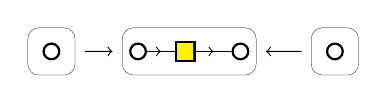
\begin{tikzpicture}
\begin{scope}[shift={(-0.5,-0.1)}]
\node [zxopen] (v2) at (1,-0.5) {};
\node (v11) at (1.3,-0.5) {};
\draw [ultra thin, rounded corners] (0.7,-0.2) rectangle (1.3,-0.8);
\end{scope}
%
\begin{scope}[shift={(4.8,0.1)}]
\node [zxopen] (v1) at (-1.9,-0.7) {};
\node [zxopen] (v2) at (-3.2,-0.7) {};
\node [zxyellow] (v3) at (-2.6,-0.7) {};
\draw [->-] (v2) to (v3);
\draw [->-] (v3) to (v1);
\draw [ultra thin, rounded corners] (-3.4,-0.4) rectangle (-1.7,-1);
\node (v12) at (-3.4,-0.7) {};
\node (v14) at (-1.7,-0.7) {};
\end{scope}
%
\begin{scope}[shift={(5.8,-0.5)}]
\node [zxopen] (v1) at (-1.7,-0.1) {};
\draw [ultra thin, rounded corners] (-2,0.2) rectangle (-1.4,-0.4);
\node (v13) at (-2,-0.1) {};
\end{scope}
%
\draw [->] (v11) edge (v12);
\draw [->] (v13) edge (v14);
\end{tikzpicture}
%
%
%
\quad \quad \quad 
%
% diamond
%
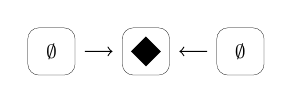
\begin{tikzpicture}
\begin{scope}[shift={(0,-0.1)}]
\node (v2) at (1,-0.5) {\scriptsize $\emptyset$};
\node (v11) at (1.3,-0.5) {};
\draw [ultra thin, rounded corners] (0.7,-0.2) rectangle (1.3,-0.8);
\end{scope}
%
\begin{scope}[shift={(4.8,0.1)}]
\node [zxdiamond] (v3) at (-2.6,-0.7) {};
\draw [ultra thin, rounded corners] (-2.9,-0.4) rectangle (-2.3,-1);
\node (v12) at (-2.9,-0.7) {};
\node (v14) at (-2.3,-0.7) {};
\end{scope}
%
\begin{scope}[shift={(5.1,-0.5)}]
\node (v1) at (-1.7,-0.1) {\scriptsize $\emptyset$};
\draw [ultra thin, rounded corners] (-2,0.2) rectangle (-1.4,-0.4);
\node (v13) at (-2,-0.1) {};
\end{scope}
%
\draw [->] (v11) edge (v12);
\draw [->] (v13) edge (v14);
\end{tikzpicture}
\]
\[
%
% green spider
%
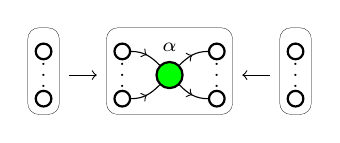
\begin{tikzpicture}
\begin{scope}[shift={(-1.4,0.1)}]
\node [zxopen] (v2) at (1.2,-0.9) {};
\node [zxopen] (v3) at (1.2,-0.3) {};
\node (v3) at (1.2,-0.5) {\scriptsize $\vdots$};
\node (v11) at (1.4,-0.6) {};
\draw [ultra thin, rounded corners] (1,0) rectangle (1.4,-1.1);
\end{scope}
%
\begin{scope}[shift={(4.1,-0.1)}]
\node [zxgreen,label={\scriptsize $\alpha$}] (v1) at (-2.7,-0.4) {};
\node [zxopen] (v2) at (-3.3,-0.1) {};
\node [zxopen] (v3) at (-2.1,-0.1) {};
\node [zxopen] (v4) at (-3.3,-0.7) {};
\node [zxopen] (v5) at (-2.1,-0.7) {};
\node at (-2.1,-0.3) {\scriptsize $\vdots$};
\node at (-3.3,-0.3) {\scriptsize $\vdots$};
\draw [->-] (v2) to [out=0,in=135] (v1);
\draw [->-] (v1) to [out=45,in=180] (v3);
\draw [->-] (v4) to [out=0,in=225] (v1);
\draw [->-] (v1) to [out=-45,in=180] (v5);
\draw [ultra thin, rounded corners] (-3.5,0.2) rectangle (-1.9,-0.9);
\node (v12) at (-3.5,-0.4) {};
\node (v14) at (-1.9,-0.4) {};
\end{scope}
%
\begin{scope}[shift={(4.8,-0.5)}]
\node [zxopen] (v1) at (-1.8,-0.3) {};
\node [zxopen] (v2) at (-1.8,0.3) {};
\node at (-1.8,0.1) {\scriptsize $\vdots$};
\draw [ultra thin, rounded corners] (-2,0.6) rectangle (-1.6,-0.5);
\node (v13) at (-2,0) {};
\end{scope}
%
\draw [->] (v11) edge (v12);
\draw [->] (v13) edge (v14);
\end{tikzpicture}
%
%
%
\quad \quad \quad \quad \quad \quad 
%
% red spider
%
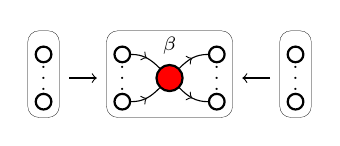
\begin{tikzpicture}
\begin{scope}[shift={(-1.4,0.1)}]
\node [zxopen] (v2) at (1.2,-0.9) {};
\node [zxopen] (v3) at (1.2,-0.3) {};
\node (v3) at (1.2,-0.5) {\scriptsize $\vdots$};

\node (v11) at (1.4,-0.6) {};
\draw [ultra thin, rounded corners] (1,0) rectangle (1.4,-1.1);
\end{scope}
%
%
%
\begin{scope}[shift={(4.1,-0.1)}]
\node [zxred,label={\scriptsize $\beta$}] (v1) at (-2.7,-0.4) {};
\node [zxopen] (v2) at (-3.3,-0.1) {};
\node [zxopen] (v3) at (-2.1,-0.1) {};
\node [zxopen] (v4) at (-3.3,-0.7) {};
\node [zxopen] (v5) at (-2.1,-0.7) {};
\node at (-2.1,-0.3) {\scriptsize $\vdots$};
\node at (-3.3,-0.3) {\scriptsize $\vdots$};
\draw [->-] (v2) to [out=0,in=135] (v1);
\draw [->-] (v1) to [out=45,in=180] (v3);
\draw [->-] (v4) to [out=0,in=225] (v1);
\draw [->-] (v1) to [out=-45,in=180] (v5);
\draw [ultra thin, rounded corners] (-3.5,0.2) rectangle (-1.9,-0.9);
\node (v12) at (-3.5,-0.4) {};
\node (v14) at (-1.9,-0.4) {};
\end{scope}
%
%
%
\begin{scope}[shift={(4.8,-0.5)}]
\node [zxopen] (v1) at (-1.8,-0.3) {};
\node [zxopen] (v2) at (-1.8,0.3) {};
\node at (-1.8,0.1) {\scriptsize $\vdots$};
\draw [ultra thin, rounded corners] (-2,0.6) rectangle (-1.6,-0.5);
\node (v13) at (-2,0) {};
\end{scope}
%
%
%
\draw [->] (v11) edge (v12);
\draw [->] (v13) edge (v14);
\end{tikzpicture}
\]  
in $\cat{zxRewrite}$.  The relations obeyed by the $\cat{zx}$-morphisms are weakened from equations to rewrite rules, which we illustrate here with equation \eqref{diag:spider relation}:
\[
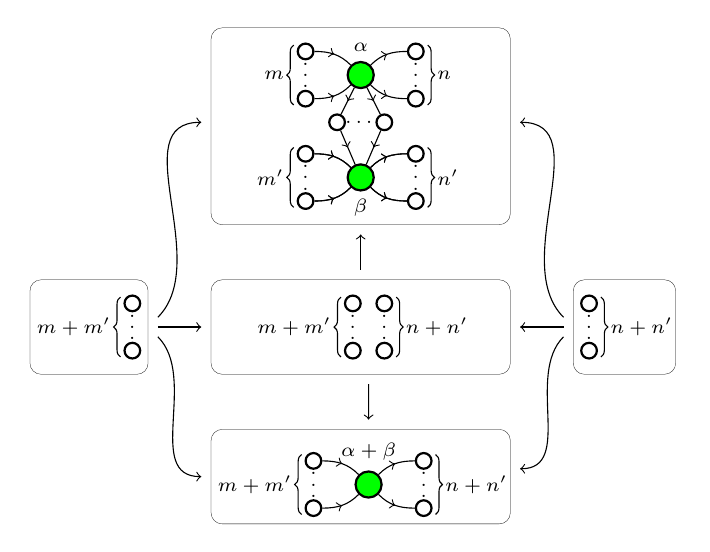
\begin{tikzpicture}
\begin{scope}[shift={(7.7,-0.1)}]
\node [zxopen] (v2) at (-3.3,0.5) {};
\node [zxopen] (v4) at (-3.3,-0.1) {};
\node at (-3.3,0.3) {\scriptsize $\vdots$};
%
\draw [ultra thin, rounded corners] (-3.5,0.8) rectangle (-2.2,-0.4);
\draw[decoration={brace,raise=2pt},decorate]
(v2.north east) -- node [right=2pt] {\scriptsize $n+n'$} (v4.south east); 
\end{scope}
%
%
%
\begin{scope}[shift={(-1.5,-0.1)}]
\node [zxopen] (v1) at (0.1,0.5) {};
\node [zxopen] (v3) at (0.1,-0.1) {};
\node at (0.1,0.3) {\scriptsize $\vdots$};
%
\draw [ultra thin, rounded corners] (-1.2,0.8) rectangle (0.3,-0.4);
\draw[decoration={brace,mirror,raise=2pt},decorate]
(v1.north west) -- node [left=2pt] {\scriptsize $m+m'$} (v3.south west);
\end{scope}
%
%
%
\begin{scope}[shift={(2.4,3.3)}]
\node [zxgreen,label={\scriptsize $\alpha$}] (v1) at (-0.9,0) {};
\node [zxopen] (v2) at (-1.6,0.3) {};
\node [zxopen] (v3) at (-1.6,-0.3) {};
\node [zxopen] (v4) at (-0.2,0.3) {};
\node [zxopen] (v5) at (-0.2,-0.3) {};
\node [zxgreen,label={[shift={(0,-0.8)}]\scriptsize $\beta$}] (v6) at (-0.9,-1.3) {};
\node [zxopen] (v7) at (-1.6,-1) {};
\node [zxopen] (v8) at (-1.6,-1.6) {};
\node [zxopen] (v9) at (-0.2,-1) {};
\node [zxopen] (v10) at (-0.2,-1.6) {};
\node [zxopen] (v11) at (-1.2,-0.6) {};
\node [zxopen] (v12) at (-0.6,-0.6) {};
%
\draw [->-] (v2) to [in=135,out=0] (v1);
\draw [->-] (v3) to [in=-135,out=0] (v1);
\draw [->-] (v1) to [in=180,out=45] (v4);
\draw [->-] (v1) to [in=180,out=-45] (v5);
\draw [->-] (v7) to [in=135,out=0] (v6);
\draw [->-] (v8) to [in=-135,out=0] (v6);
\draw [->-] (v6) to [in=180,out=45] (v9);
\draw [->-] (v6) to [in=180,out=-45] (v10);
\draw [->-] (v1) to (v12);
\draw [->-] (v12) to (v6);
\draw [->-] (v1) to (v11);
\draw [->-] (v11) to [bend right=0] (v6);
\node at (-1.6,0.1) {\scriptsize $\vdots$};
\node at (-0.2,0.1) {\scriptsize $\vdots$};
\node at (-1.6,-1.2) {\scriptsize $\vdots$};
\node at (-0.2,-1.2) {\scriptsize $\vdots$};
\node at (-0.9,-0.6) {\scriptsize $\dots$};
%
\draw[decoration={brace,mirror,raise=2pt},decorate]
(v2.north west) -- node [left=2pt] {\scriptsize $m$} (v3.south west); 
\draw[decoration={brace,mirror,raise=2pt},decorate]
(v7.north west) -- node [left=2pt] {\scriptsize $m'$} (v8.south west);
\draw[decoration={brace,raise=2pt},decorate]
(v4.north east) -- node [right=2pt] {\scriptsize $n$} (v5.south east); 
\draw[decoration={brace,raise=2pt},decorate]
(v9.north east) -- node [right=2pt] {\scriptsize $n'$} (v10.south east); 
%
\node (a1) at (-0.9,-1.9) {};
\draw [ultra thin, rounded corners] (-2.8,0.6) rectangle (1,-1.9);
\end{scope}
%
%
%
\begin{scope}[shift={(3.1,-0.1)}]
\node [zxopen] (v1) at (-1.7,0.5) {};
\node [zxopen] (v2) at (-1.3,0.5) {};
\node [zxopen] (v3) at (-1.7,-0.1) {};
\node [zxopen] (v4) at (-1.3,-0.1) {};
\node at (-1.7,0.3) {\scriptsize $\vdots$};
\node at (-1.3,0.3) {\scriptsize $\vdots$};
%
\draw [ultra thin, rounded corners] (-3.5,0.8) rectangle (0.3,-0.4);
\draw[decoration={brace,mirror,raise=2pt},decorate]
(v1.north west) -- node [left=2pt] {\scriptsize $m+m'$} (v3.south west);
\draw[decoration={brace,raise=2pt},decorate]
(v2.north east) -- node [right=2pt] {\scriptsize $n+n'$} (v4.south east); 
\node (a2) at (-1.6,0.8) {};
\node (a3) at (-1.5,-0.4) {};
\end{scope}
%
%
%
\begin{scope}[shift={(1.6,-2.5)}]
\node [zxgreen,label={\scriptsize $\alpha+\beta$}] (v1) at (0,0.6) {};
\node [zxopen] (v2) at (-0.7,0.9) {};
\node [zxopen] (v3) at (-0.7,0.3) {};
\node [zxopen] (v4) at (0.7,0.9) {};
\node [zxopen] (v5) at (0.7,0.3) {};
%
\draw [->-] (v2) to [in=135,out=0] (v1);
\draw [->-] (v3) to [in=-135,out=0] (v1);
\draw [->-] (v1) to [in=180,out=45] (v4);
\draw [->-] (v1) to [in=180,out=-45] (v5);
\draw [->-] (v7) to [in=135,out=0] (v6);
\draw [->-] (v8) to [in=-135,out=0] (v6);
\draw [->-] (v6) to [in=180,out=45] (v9);
\draw [->-] (v6) to [in=180,out=-45] (v10);
\node at (-0.7,0.7) {\scriptsize $\vdots$};
\node at (0.7,0.7) {\scriptsize $\vdots$};
%
\draw[decoration={brace,mirror,raise=2pt},decorate]
(v2.north west) -- node [left=2pt] {\scriptsize $m+m'$} (v3.south west); 
\draw[decoration={brace,raise=2pt},decorate]
(v4.north east) -- node [right=2pt] {\scriptsize $n+n'$} (v5.south east); 
%
\draw [ultra thin, rounded corners] (-2,1.3) rectangle (1.8,0.1);
\node (a4) at (0,1.3) {};
\end{scope}
%
%
%
\draw [<-] (a1) edge (a2);
\draw [->] (a3) edge (a4);
\node (a5) at (-1.2,0.1) {};
\node (a6) at (-0.4,2.7) {};
\node (a7) at (-0.4,0.1) {};
\node (a8) at (-0.4,-1.8) {};
\draw [->] (a5) to [in=180,out=45] (a6);
\draw [->] (a5) to (a7);
\draw [->] (a5) to [in=180,out=-45] (a8);
\node (a9) at (4.2,0.1) {};
\node (a10) at (3.4,2.7) {};
\node (a11) at (3.4,0.1) {};
\node (a12) at (3.4,-1.7) {};
\draw [->] (a9) edge [in=0,out=135] (a10);
\draw [->] (a9) edge (a11);
\draw [->] (a9) edge [in=0,out=-135] (a12);
\end{tikzpicture}
\]


The bicategory $\cat{zxRewrite}$ is too big to categorify $\cat{zx}$.  Instead, consider the symmetric monoidal and compact closed sub-bicategory $\bicat{zx}$ of $\cat{zxRewrite}$ that is generated by the $1$-cells and $2$-cells corresponding to the morphisms and their relations of $\cat{zx}$.  Our claim is that $\bicat{zx}$ categorifies $\cat{zx}$.  To justify this, we first define the category $\decat (\bicat{zx})$ to have as objects the $0$-cells of $\bicat{zx}$ and as morphisms the $1$-cells of $\bicat{zx}$ modulo the equivalence relation given by: $f \sim g$ if and only if there is a $2$-cell $f \Rightarrow g$ in $\bicat{zx}$.  A dagger compact structure to $\decat (\bicat{zx})$ is given \cite[Thm.~5.3]{CicalaCatZxCalc} and the main result \cite[Thm.~5,4]{CicalaCatZxCalc} provides an equivalence of dagger compact categories $\cat{zx} \to \decat \bicat{zx}$.

\bibliographystyle{eptcs}
%\bibliographystyle{plain}
\bibliography{generic}
\end{document}
